\documentclass[11pt,a4paper]{article}
\title{Assignment 2: Final Report \\ \large Interaction Technology (B3IT)}
\author{Egor Dmitriev}
\date{\today}
\usepackage[square,sort,comma,numbers]{natbib}
\usepackage{tikz}
\usepackage{graphicx} 
\usepackage{subcaption} 
\usepackage{gensymb}
\usepackage{textcomp}
\usepackage{siunitx}

\usetikzlibrary{fit, calc, arrows, positioning,chains, decorations.pathreplacing, decorations.pathmorphing}
\graphicspath{{images/}}
\begin{document}

\maketitle

\begin{abstract}
This paper features an extended discussion on the design of an automatic plant watering device with capabilities to act on its own or the use of 2D visual gesture recognition.
\end{abstract}
\newpage

\tableofcontents
\newpage

\section{Introduction}
In this paper the design of the automatic plant watering device is discussed. First in section \textit{Embedded System Design} will be discussed how the device is physically built and the functionality of it's firmware. Then we will discuss the best way to implement 2D gesture recognition using computer vision. In the final section the tests will be discussed which were performed to test the device.

\section{Embedded System Design}
This section explains how to create the automatic plant watering device, which is intelligent enough to keep itself the plant alive, while still allowing user input and providing insight on the condition of the plant itself.

\subsection{Hardware}
Materials used for the hardware design for the device are from the Iot kit.

\begin{center}
\begin{tabular}{ |l|l| } 
\hline
Amount & Material \\
\hline
1 & NodeMCU ESP8266 development board \\ 
1 & Soil moisture sensor \\ 
1 & BME280 Pressure, temperature and humidity sensor \\ 
1 & OLED display, 0.96″, 128×64 \\
1 & Micro servo \\
1 & Custom Analog multiplexer SMD \\
1 & LDR Light dependent resistor \\
\hline
\end{tabular}
\end{center}
\bigskip

To create the final device the OLED display and BME280 sensor were connected to the ESP8211. Pins number D5 and D3 were used to connect them the SCL and SDA pins which are used to run the I2C protocol.
\newline
After that the LDR and soil moisture sensor are both attached to the custom analog multiplexer board which itself is connected to analog pin 0 and the digital pin 4 to switch between the two sensors.
\newline
Finally the servo is connected the ESP8633 with the digital pwm pin 6 as control pin.\bigskip

The device used by moving it beside the plant so the temperature, air moisture and light exposure are similar to what is measured around the plant. The soil moisture sensor is then carefully placed inside the plant pot so no roots are hit. The servo is attached to a straw which is connected to a filled water bottle. The straw should attached be at 12 hours angle when its resting and directed to the plant pot so when the straw is turned 90 degrees it will be right above the soil the plant is in.

\subsection{System Architecture}
While designing the architecture for the firmware of the device extensibility and non blocking task execution has played a played a huge role. This is needed because the OLED screen, MQTT client and WIFI need to be able to run in the background. Therefore the created scheduler library which was used for the previous assignment was reused.\bigskip

\subsubsection{Scheduler and tasks}
To add extensibility to the firmware I have split every function of the device into a task which is either scheduled to run at an interval or when certain conditions are met. A high level representation of the used structure can be seen in figure~\ref{fig:deviceSchedule}. Because every task is scheduled to run at a certain interval no delays are required and system is thus non blocking.\bigskip

\begin{figure}
\begin{center}
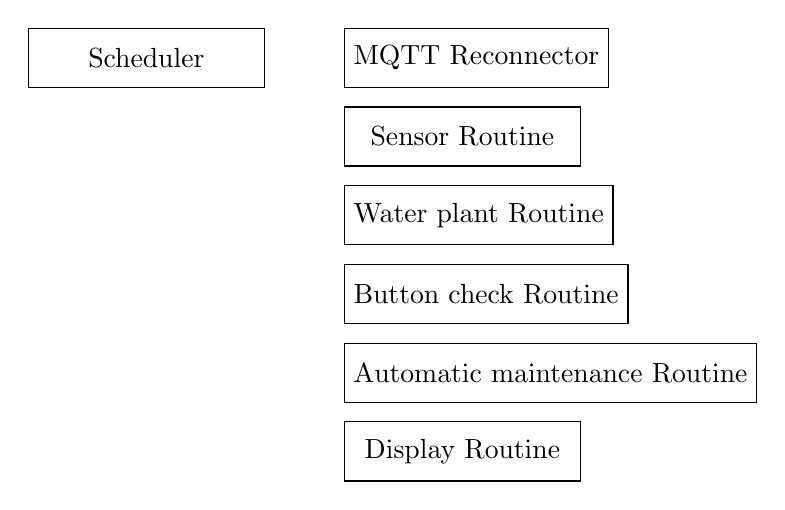
\begin{tikzpicture}[auto, node distance=1cm,>=latex']
      node distance=3cm] (system) {System};
\tikzset{
    box/.style={draw=black,minimum width=3cm,minimum height=.75cm},
    >=latex,
  }
\node (scheduler) [box] {Scheduler};
\node (mqtt_task) [box, right=of scheduler] {MQTT Reconnector};
\node (sensor_task) [box, below=of mqtt_task.west,anchor=west]  {Sensor Routine};
\node (water_task) [box, below=of sensor_task.west,anchor=west] {Water plant Routine};
\node (button_task) [box, below=of water_task.west,anchor=west] {Button check Routine};
\node (maintenance_task) [box, below=of button_task.west,anchor=west] {Automatic maintenance Routine};
\node (display_task) [box, below=of maintenance_task.west,anchor=west] {Display Routine};
\end{tikzpicture}
\end{center}
\caption{Architecture of the device}
\label{fig:deviceSchedule}
\end{figure}

\begin{description}
\item [MQTT Reconnector Routine] is responsible for keeping the MQTT connection up to date. If every five seconds the task is run to check if the connection with MQTT broker is lost. On connection loss the device will try to reconnect. If device still could not connect successfully the process will be repeated after another 5 seconds.
\item [Sensor Routine] is scheduled to run every two seconds to poll the sensor measurements and publish them using the MQTT client. Measurements will also be stored in the store where all the tasks can access the values.
\item [Water plant Routine] is run only when it is requested to by other tasks or a request of MQTT subscription handler. It is responsible for the whole plant watering cycle. It can run a customized amount of time. 50\% of the watering time will be spent lowering and holding the watering straw down using the servo motor. The other 50\% will be spent raising the straw back up.
\item [Button check Routine] is used to check if the on board flash button is pressed. If it is, then the automatic mode will toggled. The result will be published using MQTT client. Because the task is run regularly but not every tick, this also acts as a debounce.
\item [Display Routine] is responsible for displaying and animating different slides five seconds. There four different slides of which three cycle in a loop and display measurements and device state, while the fourth one only becomes visible when device is watering the plants and contains a progress bar to indicate its state.
\end{description}

\subsubsection{Stores}
Every task can access the other tasks to invoke some kind of action of read it's state. For more global information \textbf{store} is used to write data to. There are two kind of stores used: 

\begin{description}
\item [Config] \textit{(Config store)} which contains all the data which is configured via administration panel which can be accessed by vising the IP address of the device on port 80. Config store is synchronized with EEPROM and is therefore preserved if device is turned off. 
\item [Sensor data] \textit{(Sensor data store)} contains all the sensor measurements and  relevant data like timestamp when the plants last have been watered.
\end{description}

As stated earlier the administrative UI (figure \ref{fig:adminPanel}) is used when to adjust configuration. On initial start if no last connected WIFI network is found the devices goes into \textbf{Access Point} mode and allows user to fill the new WIFI information first. After thet the full configuration menu is shown where user can adjust various settings like MQTT credentials. On save settings are sent via \textbf{REST} requests to the device.

\begin{figure}
\begin{center}
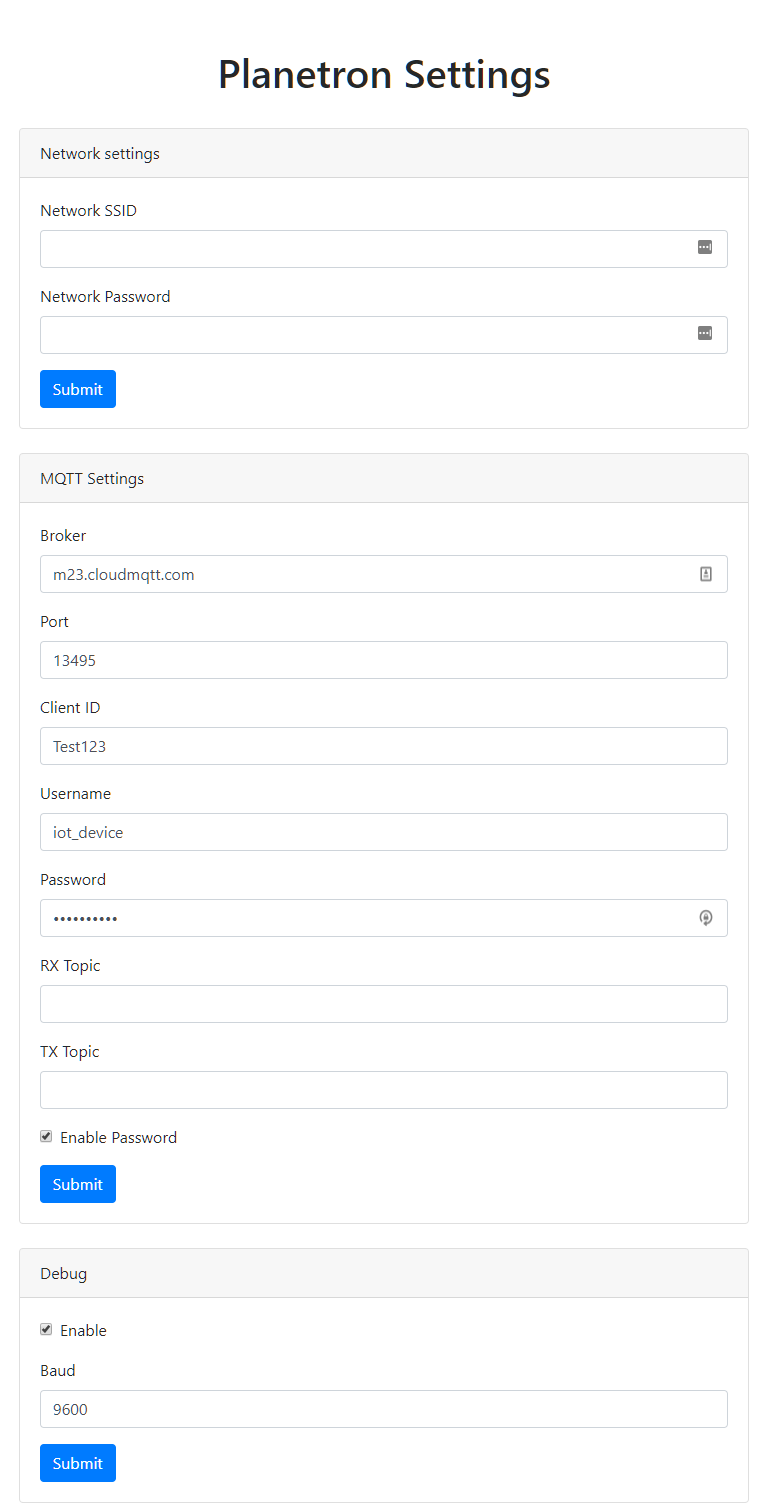
\includegraphics[scale=0.35]{admin_panel}
\end{center}
\caption{Admin panel}
\label{fig:adminPanel}
\end{figure}

\subsubsection{MQTT client}
An external library is used to maintain connection with PubSubClient. Connection maintained by \textbf{MQTT Reconnector Routine} task.\bigskip

On every connection request \textbf{last will} is attached to the headers by the task. This last will sends a zero character payload to the topic "\dots/status/alive" with retain flag as true and quality of service 2. By doing this broker notifies everyone subscribed that given device is offline. Naturally, when the device is connected it will publish a character one to the same topic and retain flag to let the subscribed clients know that it is alive.\bigskip

Aside from bragging about it's sensor measurements the device is also subscribed to multiple different topics on connection including "plant watering", "force refresh measurements" and "toggle automatic mode" topics. Callback for this topic is also inside the scheduler but not as a task. Instead its a callback function attached to the scheduler instance which gets called by MQTT client.\\In the callback function the topic and its payload are matched to the given intent. Additionally if intent is to toggle the automatic mode on or off the built in led gets also updated to the corresponding state.\bigskip

Topic naming is quite intuitive and always uses \textit{"devices/assignment\_device/"} as root to maintain extensibility if more devices are needed. From there there are two topic groups \textit{"interaction"} which contains all the topics which are interactive like topic to start watering the plants and there is a topic group \textit{"sensors"} which is root for all the sensor topics which device publishes. A example few topics would be:

\begin{center}
devices/assignment\_device/sensor/temperature\\
devices/assignment\_device/sensor/alive\\
devices/assignment\_device/interaction/automatic\_mode\\
\end{center}

\subsubsection{Libraries}
A few external libraries were used for this assignment. First of all the platformio build platform was used to create and compile the project. Instead of using sketches it compiles standard C++ .cpp and .h files which makes code easier to see (\textbf{Note: because of this code is submitted instead of the sketch file. I hope that is not an issue. It can easy be compiled by installing: https://platformio.org/ and pointing it to platformio.ini}). Also it downloads the needed libraries stated below.

\begin{description}
\item[EEPROM]
\item[PubSubClient] For mqtt support]
\item[Wire] To use the arduino sensors that work with IC2
\item[ESP8266\_SSD1306] To use the OLED screen
\item[Adafruit\_Sensor] To use the multisensor for temperature and pressure. Its a dependency for Adafruit\_BME280\_Library
\item[ConfigManager] To automatically reconnect to wifi and act as server to display admin panel.
\item[Adafruit\_BME280\_Library]To use the multisensor for temperature and pressure
\item[DNSServer] Dependency for ConfigManager
\item[Servo] To control the servo
\end{description}


\subsection{External integration}
As stated in the assignment requirements some external tools are also integrated in the whole device stack. The broker is being hoster on the MQTT cloud.

\subsubsection{Node Red}
I have created a Node Red flow graph to create a MQTT client which can interact with the device and read it's measurements.\bigskip

Flow graph starts at the entry MQTT node which is subscribed to all sensors and interactive topics using the wildcard \# \textit{"devices/assignment\_device/\#"}. Then the output of MQTT node goes into the topic switcher where different topics are matched and their payloads are passed to the correct output. At each output there are UI nodes which are from "node-red-dashboard" library. These nodes display the input data. The flowchart can be seen in figure \ref{fig:nodeRed} and the dashboard in figure \ref{fig:nodeRedDash}.

\begin{figure}
\begin{center}
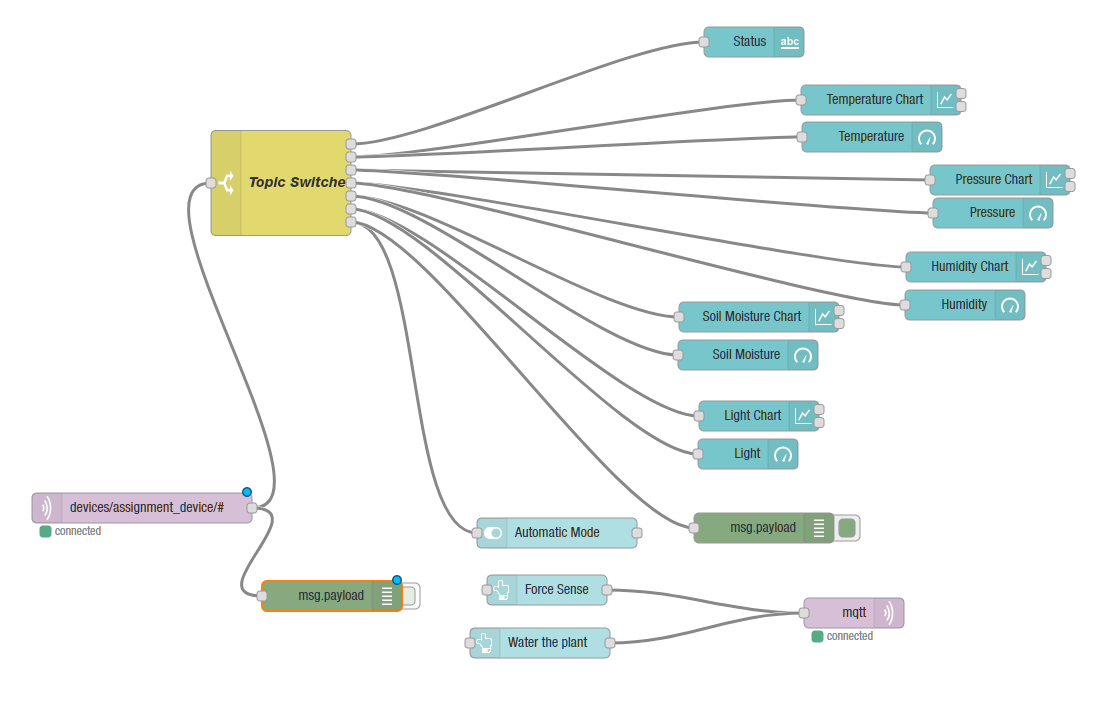
\includegraphics[scale=0.52]{node_red}
\end{center}
\caption{Node red flowchart}
\label{fig:nodeRed}
\end{figure}

\begin{figure}
\begin{center}
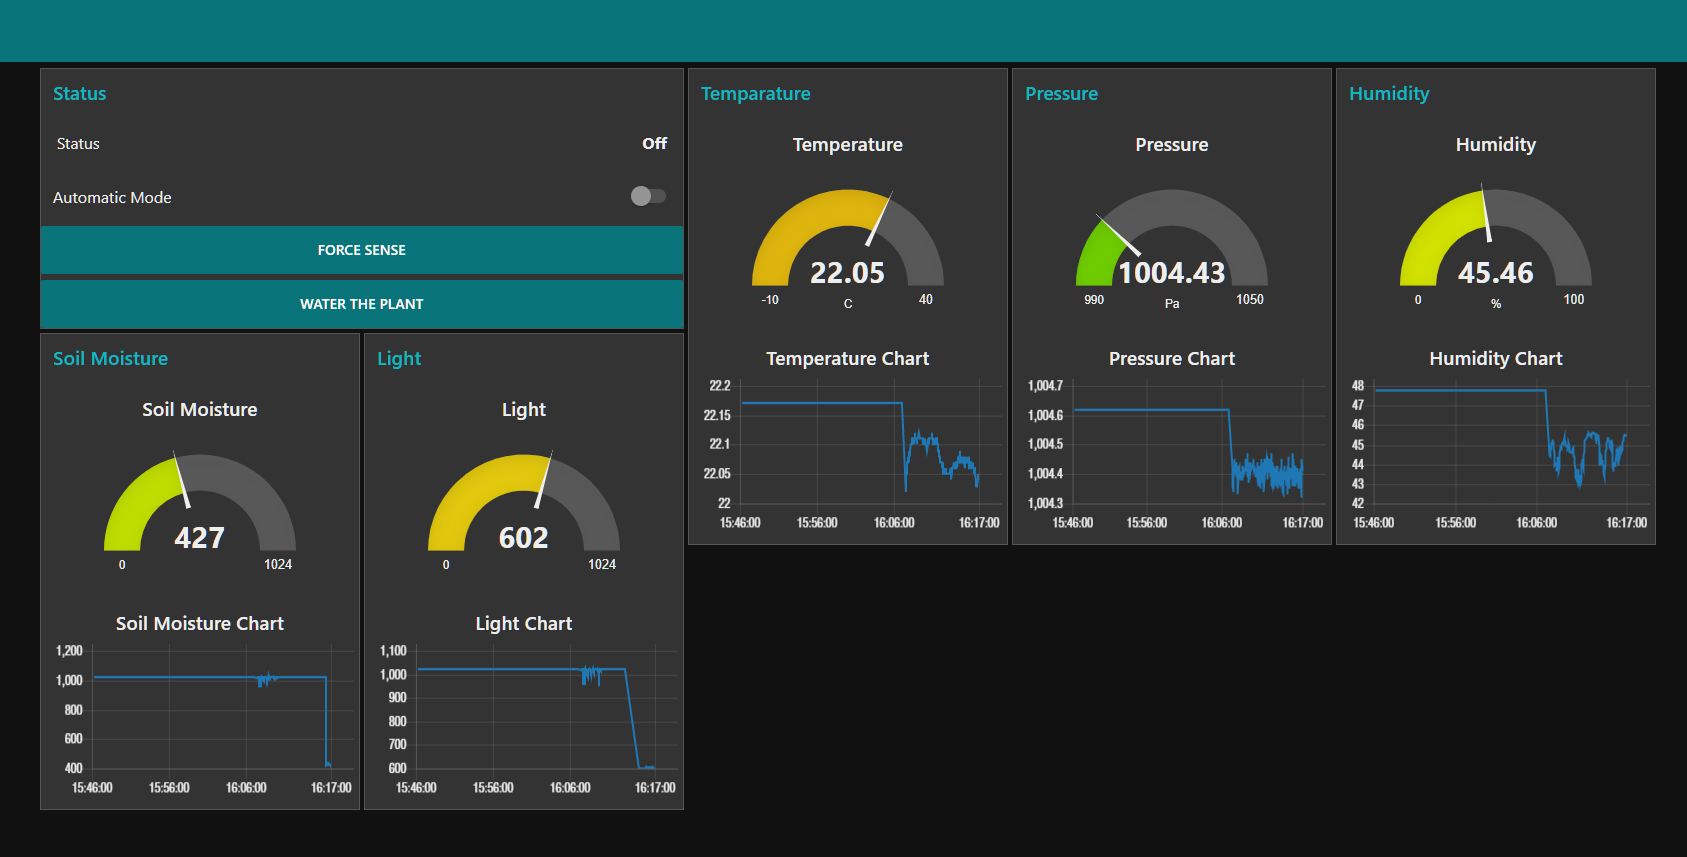
\includegraphics[scale=0.3]{node_red_panel}
\end{center}
\caption{Node red dashboard}
\label{fig:nodeRedDash}
\end{figure}

\subsubsection{MQTT.fx}
The MQTT messages can also be monitored from desktop pc with a MQTT client. MQTT.fx in this case (figure \ref{fig:mqttFX}). 

\subsection{MQTT buddy}
The MQTT messages can also be monitored from mobile with a MQTT client. MQTT buddy in this case (figure \ref{fig:mqttBuddy}). It is interactive and can display control the device like watering the plants and mode switching with a click of a button.

\begin{figure}
\begin{subfigure}[h]{0.65\linewidth}
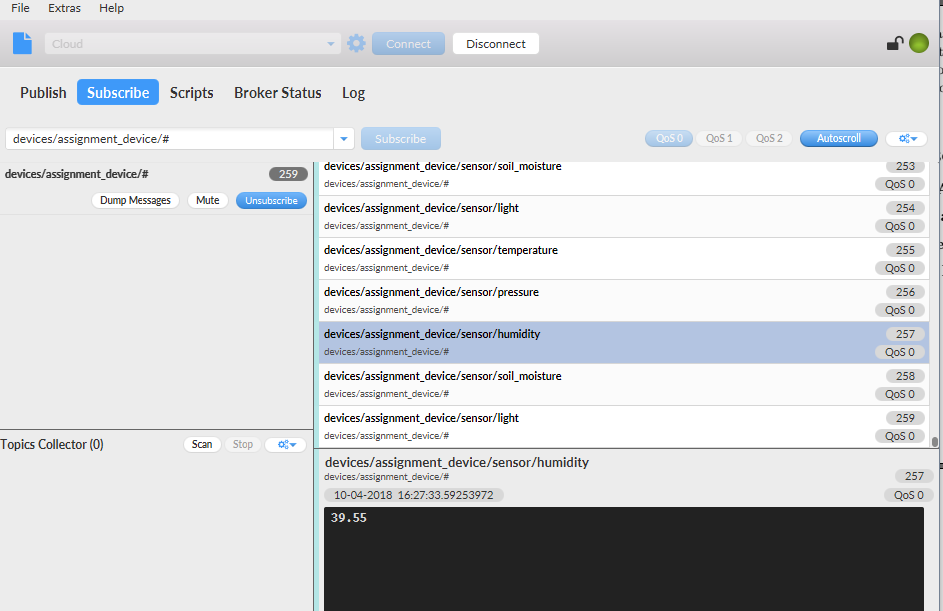
\includegraphics[width=\linewidth]{mqtt_fx}
\caption{MQTT.fx window}
\label{fig:mqttFX}
\end{subfigure}
\hfill
\begin{subfigure}[h]{0.3\linewidth}
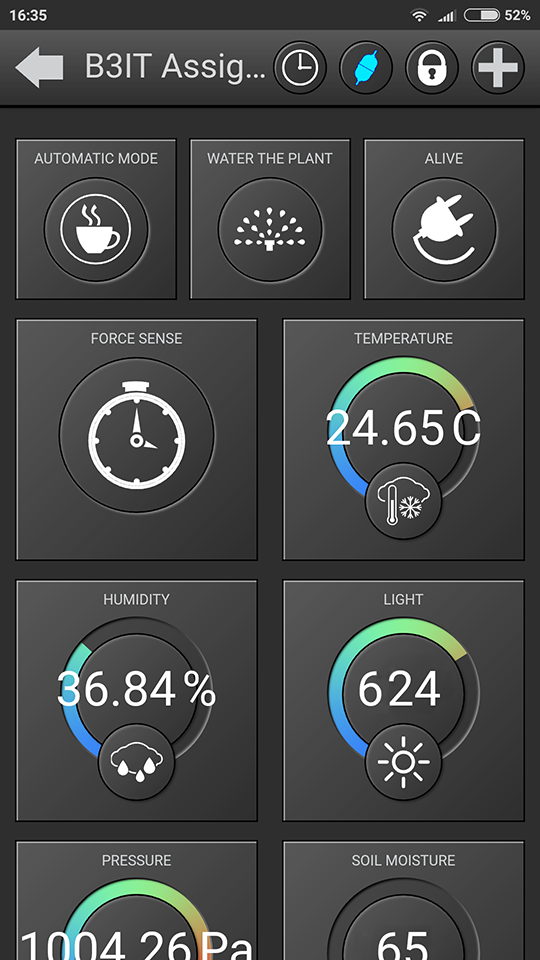
\includegraphics[width=\linewidth]{mqtt_buddy}
\caption{MQTT Buddy}
\label{fig:mqttBuddy}
\end{subfigure}%
\end{figure}

\section{Computer Vision}
Second part of the device is a client with a running program which can perform gesture recognition on given webcam video feed and send corresponding commands to the device itself to perform action. In following sections I will explain how extracting gestures from a 2D images is implemented. 

\subsection{System Architecture}
First of all the program is split into two parts:\textbf{\textit{"cvision"}} library which should not be confused with \textit{"cv/opencv"} library and the \textbf{main} ui. 

\begin{description}
\item [cvision] is created for this assignment but is meant to be reused with other projects. It has implementations of general methods for histogram extraction, image segmentation, limb recognition and object tracking. OpenCV library is used to achieve that.
\item [main] consists of a collection of ui components and a defined order in which the different features of cvision are used. 
\end{description}

User UI exists of a window and a ordered set of different components named \textbf{window helpers}. Window rendering starts by creating an empty image matrix and passing it in order to every window helper which can draw on it or swap it for another image matrix. With this the whole gesture recognition task is broken in a set of small tasks. One helper is responsible for task of segmenting the image while the other is responsible for cleaning the segmented mask. Window helpers are also interconnected and can pass data between each other (For example: segmentation helper passes mask to segmentation cleaner). The whole flow can seen in figure \ref{fig:windowFlow}.\bigskip

\begin{figure}

%TODO: explain layers
\begin{center}
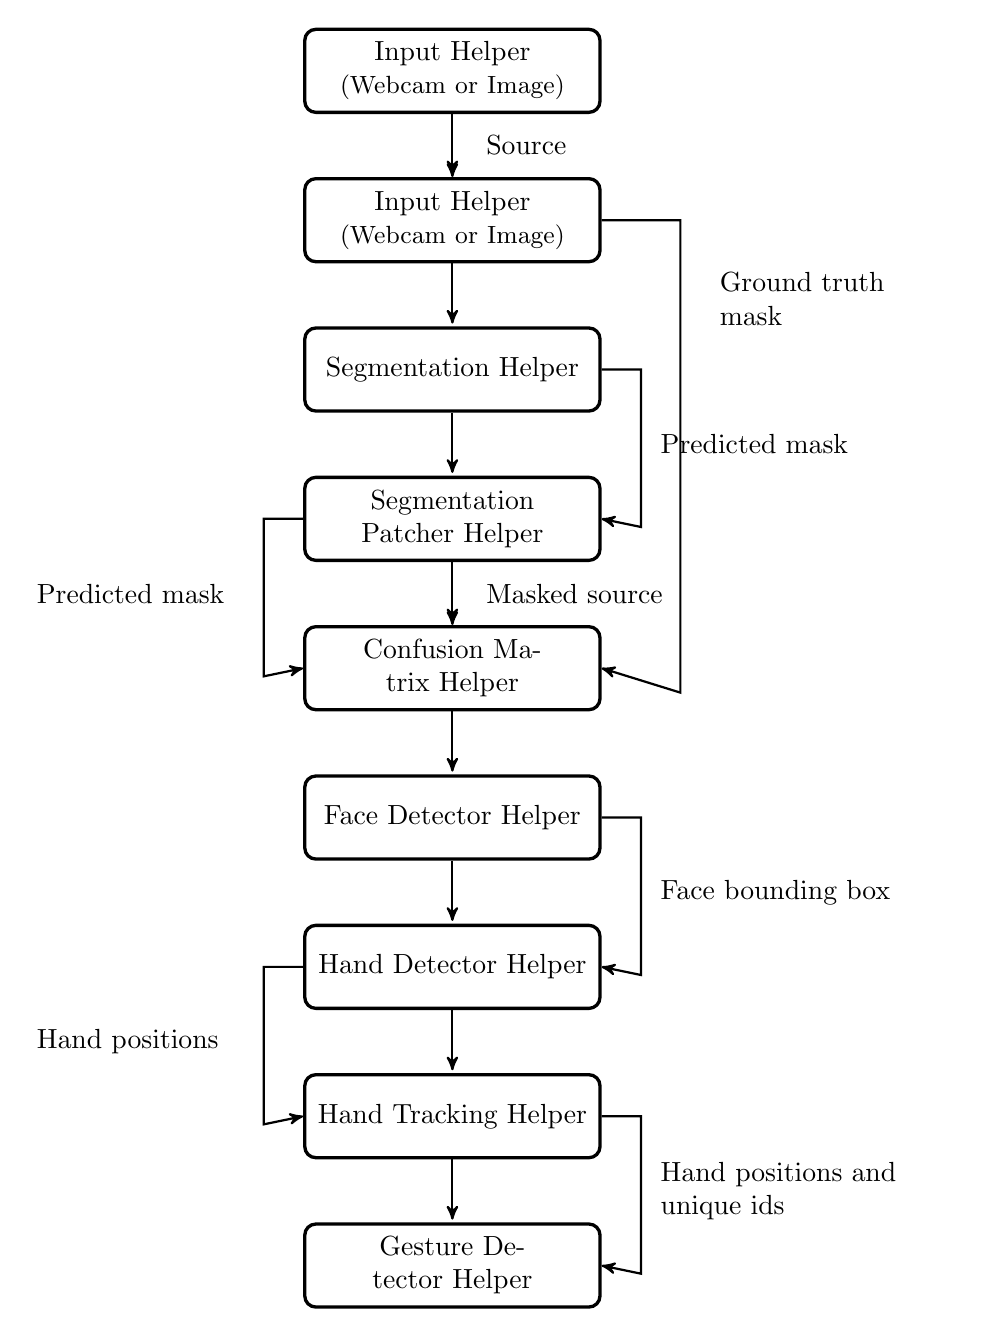
\begin{tikzpicture}[node distance=.8cm, start chain=going below,]
\tikzset{
>=stealth',
  punktchain/.style={
    rectangle, 
    rounded corners, 
    % fill=black!10,
    draw=black, very thick,
    text width=10em, 
    minimum height=3em, 
    text centered, 
    on chain},
  line/.style={draw, thick, <-},
  element/.style={
    tape,
    top color=white,
    bottom color=blue!50!black!60!,
    minimum width=8em,
    draw=blue!40!black!90, very thick,
    text width=10em, 
    minimum height=3.5em, 
    text centered, 
    on chain},
  every join/.style={->, thick,shorten >=1pt},
  decoration={brace},
  tuborg/.style={decorate},
  tubnode/.style={midway, right=2pt},
}
\node[punktchain, join] (source) {Input Helper\\\small{(Webcam or Image)}};
\node[punktchain, join] (mask) {Input Helper\\\small{(Webcam or Image)}};
\node[punktchain, join] (segmentation) {Segmentation Helper};
\node[punktchain, join] (patcher) {Segmentation Patcher Helper};
\node[punktchain, join] (cf) {Confusion Matrix Helper};
\node[punktchain, join] (face) {Face Detector Helper};
\node[punktchain, join] (hand) {Hand Detector Helper};
\node[punktchain, join] (tracking) {Hand Tracking Helper};
\node[punktchain, join] (gesture) {Gesture Detector Helper};

\draw[->, thick,] (segmentation.east) 
-- ++(0.5,0) -- ++(0,-2) -- 
node[xshift=2cm,yshift=1cm, text width=3cm] {Predicted mask} 
(patcher.east);

\draw[->, thick,] (patcher.west) 
-- ++(-0.5,0) -- ++(0,-2) -- 
node[xshift=0cm,yshift=1cm, text width=3cm,anchor=east] {Predicted mask} 
(cf.west);

\draw[->, thick,] (face.east) 
-- ++(0.5,0) -- ++(0,-2) -- 
node[xshift=2cm,yshift=1cm, text width=3cm] {Face bounding box} 
(hand.east);

\draw[->, thick,] (hand.west) 
-- ++(-0.5,0) -- ++(0,-2) -- 
node[xshift=0cm,yshift=1cm, text width=3cm,anchor=east] {Hand positions} 
(tracking.west);

\draw[->, thick,] (tracking.east) 
-- ++(0.5,0) -- ++(0,-2) -- 
node[xshift=2cm,yshift=1cm, text width=3cm] {Hand positions and unique ids} 
(gesture.east);

\draw[->, thick,] (mask.east) 
-- ++(1,0) --
node[xshift=2cm,yshift=2cm, text width=3cm] {Ground truth mask} 
++(0,-6) -- 
(cf.east);

\draw[->, thick,] (source) --
node[xshift=0.3cm,yshift=0cm, text width=3cm, anchor=west] {Source} 
(mask);

\draw[->, thick,] (patcher) --
node[xshift=0.3cm,yshift=0cm, text width=3cm, anchor=west] {Masked source} 
(cf);


\end{tikzpicture}
\end{center}
\caption{Structure of window helpers for gesture recognition task}
\label{fig:windowFlow}
\end{figure}

The final image is then drawn by the window helper. Before that the image is passed between different helpers that either modify it, do nothing or draw some debug information. The convention is not to modify the image if it should not be visible in the final result to avoid building of a unorganized flow (Passing masks as result image to next layer is prohibited. Instead it is accessed by the layer that needs it). \bigskip

Every

\subsubsection{Performance}
The performance was kept in mind when creating all the layers and segmentation. Therefore calculating the bayes probability per pixel is happening in parallel. \textit{(file: cvision/segmentation.cpp method: complex\_segmentation}). For Face detection Viola Jones algorithm is used. This is provided by opencv out of the box and could not be optimized. Overal with face detection the frame render time is 50ms(20 fps) wand without 23ms(43fps) which is enough to hold a steady frame rate.

\subsection{Segmentation}
Before hand can be extracted from the image the hand itself needs to be found. Since we are working with a 2D image, it will happen by extracting the relevant color from the image which can be classified as skin color.

\subsubsection{Probabilistic skin extraction}
In order to do that two histograms are made from a dataset of images with pre-masked skin parts. First histogram the occurrences of skin colors while the other is for occurrences of non skin colors (Figure \ref{fig:histogram}). This histogram is takes values 0-255 from RGB colorspace \citep{Jones2002} and counts the sightings into the histograms. Finally the confidence of wether something is a skin and non-skin color can be used in to predict the final probability of a pixel is a skin pixel or not with Bayesian theorem (equation \ref{bayes}). If probability is larger than a certain threshold then is seen as a skin pixel. Threshold is adjustable by the user. This statistical approach of segmenting skin from images approach is borrowed from \citet{Jones2002}. This process can be found in \textit{(file: cvision/segmentation.cpp method: complex\_segmentation}) and \textit{(file: cvision/evaluation.cpp method: bayes\_probability)}

\newcommand{\nonskin}{\ensuremath{\textit{non-skin}}}%
\begin{equation}
P(skin \mid \nonskin) = \frac{P(\nonskin \mid skin) \, P(skin)}{P(\nonskin)}
\label{bayes}
\end{equation}

Extracted data is saved as a separated file which can be loaded anytime so histograms don't need to be calculated every time. File is in \textit{"data/saves/complex\_seg.save"}

\subsubsection{Morphology}
After the generation of the mask it is very noisy. This noise is removed at morphology stage of the segmentation. First erode and then dilate is applied to the mask. A kernel of size 3 px proved to provide the best results. \textit{(file: cvision/segmentation.cpp method: clean\_segmentation})

\subsubsection{Evaluation}
The results of of the masks are passed to the Confusion Matrix helper which if provied a ground truth compares the two masks and calculates the confusion matrix. The result is then logged. By evaluating the whole dataset and averaging the following results were extracted. \textbf{Note:} the validation dataset was included in the training dataset, so the results might have a slight bias. \textit{(file: cvision/evaluation.cpp method: evaluation::make\_confsion\_matrix})

\begin{center}
\begin{tabular}{ |l|l|l| }
\hline
Statistic & hgr1 dataset & Pratheepan dataset \\ 
\hline
True positives & 40.08\% & 9.31\% \\ 
True negatives & 57.31\% & 0.60\% \\ 
False positives & 1.20\% & 89.57\% \\
False negatives & 1.40\% & 0.50\% \\
Relative Error & 0.0162933 & 0.0111449 \\
Total Preformance & 0.0160321 & 0.011022 \\
Bulls eye \% & 100\% & 94.89\% \\
Precision & 96.15\% & 93.93\% \\
Recall & 100\% & 94.89\% \\
F1 score & 98.03\% & 94.41\% \\
Specificity & 97.32\% & 99.33\% \\
Generality & 40.00\% & 9.81\% \\
\hline
\end{tabular}
\end{center}

Two different datasets were used. While hgr1\citep{Kawulok2014EURASIP}\citep{Grzejszczak2016MTA} dataset has different lightning conditions and a lot of data there is not much diversity in skin color. Pratheepan\citep{Praptheepan} on contrary has a lot of diversity but very few samples.

\begin{figure}
\begin{center}
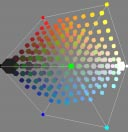
\includegraphics{histogram}
\end{center}
\caption{Skin histogram~\citet{Jones2002}}
\label{fig:histogram}
\end{figure}

\subsection{Hand Recognition}
Once skin colored pixels are segmented, the contours are created around the left over parts. If area of a contour is larger than the specified threshold then is seen as a significant candidate to be a hand.\textit{(file: main/detection\_helper.h method: HandDetectorHelper::draw})\bigskip

Face detection is used to remove corresponding contours from the candidate list and thus thinning the list. Every contour from here on is regarded as hand if it passes minimum requirements like having at least three vertices. False positives can't be efficiently eliminating without creating as large abundance of false negatives since a closed hand has not much characteristics. This is compensated by gesture recognition by initiating with some hard to falsify characteristics like presence of five fingers.\bigskip

Hand recognition works as follows.
\textit{(file: cvision/hand\_recognition.cpp method: hand::recognize\_hand)}

\subsubsection{Hand Palm extraction} 
The most reliable way to find the palm center is to fine largest incircle of the contour. Circle with palm center as center and radius 3.5 times larger than palm center is regarded as \textbf{region of interest}.\citet{Yeo2015}\bigskip

My own touch on this was adding the weight to certain areas of the contour for incircle to be found. Sometimes there is an arm attached to the hand which can produce a larger incircle than the palm itself. Therefore the convex defects in the contour will be seen as points of priority. The weight of those points is tuned to the largest incircle will be found but still nearby these points.\textit{(file: cvision/geometry.hpp method: incircle)}\bigskip

Once this palm circle is found we can cut the arm off by checking what is outside of the region of interest. If something is it is regarded as an arm and will be cut off from the palm itself and not the area of interest.\textit{(file: cvision/hand\_recognition.cpp method: hand::find\_enclosing\_circle)}

\subsection{Finding fingers}
Fingers are categorized as defects in the convex hull of the hand contour. Aside from that they are pointy and are angle constrained. These characteristics are used to locate the finger positions in the given contour.\citet{Yeo2015}\bigskip

To be more precise the following checklist used to find the fingers:
\textit{(file: cvision/hand\_recognition.cpp method: find\_fingers)}
\begin{enumerate}
\item The depth of the defect is larger than palm center radius but shorter than minimum enclosing circle radius.
\item The angle of the defect is smaller than 100\degree
\item The curvature of the tip is less than 60\degree
\end{enumerate}

The following approach is very effective for finding two fingers or more. But unfortunately it doesn't work for when only one finger is visible. Therefore there is also a fallback function if no fingers are found.
\textit{(file: cvision/hand\_recognition.cpp method: find\_fingers\_fallback)}
\begin{enumerate}
\item The depth of the defect is larger than defined threshold.
\item The curvature of the tip is less than 80
\end{enumerate}

\begin{figure}
\begin{center}
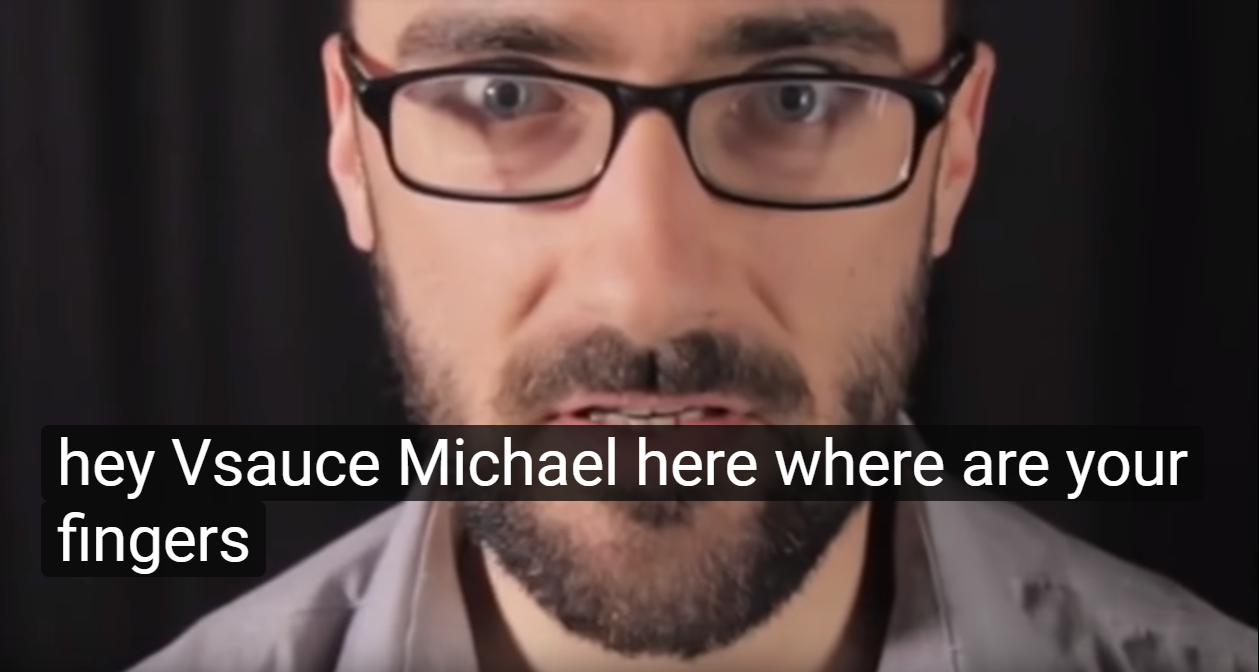
\includegraphics[scale=0.3]{fingers}
\end{center}
\caption{Where are your fingers? Vsauce}
\label{fig:fingers}
\end{figure}

Finally when fingers are found the fingertip is extracting by finding the smallest curvature point. Form there the x amount of points to the left and right in the contour are taken, summed up and divided by two which finds a point in the centre of the finger. Now since we have two points the direction can be estimated. Points on the same finger should point to the same peak. If they don't they are still near each other and are removed if the distance between them is smaller than the 0.75 * finger width.\textit{(file: cvision/hand\_recognition.cpp method: remove\_duplicate\_fingers)}

\begin{figure}
\begin{center}
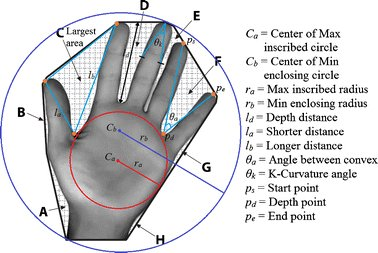
\includegraphics{hand_fingers}
\end{center}
\caption{Convex hull, convexity defects of hand shape, extracted from \citep{Yeo2015} Learning OpenCV}
\label{fig:histogram}
\end{figure}

All the fingers and hand information are then stored in a struct which can be further analyzed on.

\subsection{Gesture Recognition}
\subsubsection{Hand Tracking}
In order to track the hand gestures we first need to be able to identify the instanced of the same hand in multiple different images. For this the so called nearest neighbor matching is used. The hand positions are saved inside the history every frame. On the new frame the hands are again found. To find which instance this hand belongs to all centers the hands in the frame are taken en the nearest neighbor to it is found using the following algorithm:\textit{(file: cvision/object\_tracking.cpp method: match\_points)}\bigskip

\begin{enumerate}
\item All new points are tupled with the most recent points in history, distance is calculated and the tuple stored in an array.
\item Array is sorted on distance
\item The first(with shortest distance) tuple in the array is taken and the two corresponding instances are a match (they belong to the same object).
\item All the in tuples containing any of the two points are removed from the array. And step two is repeated untill array is empty.
\end{enumerate}

After that the objects that have no history are added and ones that don't exists anymore have their history removed. To add bit more leniency in this step a time out is used. If object is not present for x steps anymore then is removed. Same goes for new objects, only if their history >x entries long they are considered relevant.\textit{(file: cvision/object\_tracking.h method: update)}

\subsubsection{Identifying gestures}
To identify gestures I have opted in for the Dollar since it's already made and works "oke'ish". The gesture consist of three different states. \textit{(file: main/gesture\_recognition\_helper.cpp method: GestureDetectSession::update)}

\begin{description}
\item[Preparation] User states the intent to that the gesture by opening their hand and showing five fingers. (Hopefully that is not an issue ;))
\item[Stroke] User draws a shape which is later passed to the dollar recognizer. For this user should only use one finger.
\item[Termination] User shows again five fingers to confirm that the gesture is complete. If at any given moment user closes their hand so no fingers are visible, then the gesture is canceled. More on this in user evaluation.
\end{description}

The recorded location of the finger that is drawing the motion is saved and stabilized using the Kalman filter.

\section{User Evaluation}
To evaluate usability of the system a controlled test is performed. This is to evaluate how easy it is to use the gesture recognition and test a hypothesis:

\begin{center}
\textit{Terminating a gesture with an open palm and canceling with closed is more intuitive for user than vice versa.}
\end{center}

\subsection{Methods}
\subsubsection{Participants and Environment}
Participants used in this test are all within my friends and family circle. I have managed to get five people to participate in my despicable test.\bigskip

The environment used is the living room and the bedroom. Both rooms are used at different times and therefore vary in background and lighting which are the independent variables which vary and should not affect the results of the test.\bigskip

For the test itself my laptop is used which has a webcam and more than enough power to run the gesture recognition program. Also it runs Arch linux ;)

\subsubsection{Procedure and design}
Before the test all the participants are explained the working of the gesture recognition software and the two cases that will be tested.

\begin{description}
\item[Case 1] User draws three different gestures: a circle, a square and a triangle. To do that user activates the gesture by opening their and and terminates by closing it. To cancel it user can open the hand again which will activate the new motion.
\item[Case 2] User draws three different gestures: a circle, a square and a triangle. This time user closes hand to cancel the motion and opens it to terminate/confirm the motion.
\end{description}

At after each case user gets a survey with three different questions there user can answer using Likert scales. For this five options are given: strongly disagree, disagree, neutral, agree and strongly agree. After this the answers are summed up and compared.The questions that are asked.\bigskip


\begin{enumerate}
\item Drawing gestures works seamless.
\item I find myself trying to remember how to use the system.
\item Gesture drawing process feels natural.
\end{enumerate}

Aside from the survey task completion time for every gesture is measured and the amount of times user fails to draw the gesture and hast to restart.

\subsection{Results}
Firstly the survey results are analyzed. The summarization of the survey results is as following. If user strongly disagrees it is counted as -2 and if strongly agrees it is counted as 2. Of questions that ate negative the score is multiplied by -1.

\begin{center}
\begin{tabular}{ |l|l|l| }
\hline
Question & Summary Case 1 & Summary Case 2 \\
\hline
1 (positive) & 5 & 6 \\
2 (negative) & -2 & -5 \\
3 (positive) & -3 & 7 \\
\hline
total (corrected) & 4 & 18 \\
\hline
\end{tabular}
\end{center}

Because the amount of test subjects was small and thus was the population and sample size we cannot do perform Significance testing using z-Score. For this I use the t-Score. Also it is possible to calculate the confidence interval. Confidence level of 95\% is used Results can be found below:
 
\begin{center}
\begin{tabular}{ |l|l|l|l|l| }
\hline
Case & Task & Mean time & Standard Deviation & Confidence Interval \\
\hline
1 & Draw Circle & 12.3 & 1.9 & 12.3 \textpm\ 1.7 \\
1 & Draw Triangle & 14.1 & 2.7 & 14.1 \textpm\ 2.4 \\
1 & Draw Square & 16.6 & 3.2 & 16.6 \textpm\ 2.8 \\
2 & Draw Circle & 11.7 & 1.5 & 11.7 \textpm\ 1.3 \\
2 & Draw Triangle & 12.8 & 2.1 & 12.8 \textpm\ 1.8 \\
2 & Draw Square & 14.2 & 2.2 & 14.2 \textpm\ 1.9 \\
\hline
\end{tabular}
\end{center}

\subsection{Discussion}
Case 2 seems to be the better of the two judging from the results of the survey. SInce it has a higher score of 18 compared to case 1 that has score of 4. Aside from that Completion times for the gesture drawing tasks seem to be lower for case 2 which suggests that that gesture recognition flow is more intuitive. The results of question three seem to confirm that. Its seems that it is more natural to confirm with hand open and cancel a gesture with hand closed. \bigskip

With this the hypothesis seems to have been confirmed and will be used in the final version of gesture recognition system.


\section{Conclusions}
Overall the device as end result has turned out better than expected. Its very extensible, has beautiful UI and works as expected. Some more intelligence like more advanced prediction when the plant needs to be watered would be better than just checking if soil is dry or not. Some cover for the device to prevent shorts if water has been spilled would also be a great idea.\bigskip

Computer vision also turned out great and I have learned a lot making the system which I am very proud of. The extensibility because of its modular design is insane and worth saving. Aside from that i now have a library with a lot of handy implementations of different algorithms which can be reused in different projects. The skin segmentation works great on the datasets themselves but unfortunately these datasets still have very few skin data. Al through  smaller bin sizes in histograms can be used they seem to work degrading for the end results. More data is needed since in practice I have come a lot of (skin) colors which were not in both skin and non-skin histograms and therefore were giving nan when calculating the bayes probability.\bigskip

Gesture recognition worked out also fine, but dollar recognizer seems to work not very good in practice. A lot of times a cross or a triangle is detected when user is drawing a square. This can be solved by writing own better shape recognizer. Finding hands worked out also very good. Aside from a lot of true positives the real hand gets detected correctly a large portion of the time with fingers aligned correctly.

\bibliographystyle{unsrtnat}
\bibliography{refs}

\end{document}
